\documentclass[12pt, a4paper]{article}

% Packages
\usepackage[utf8]{inputenc}
\usepackage[T1]{fontenc}
\usepackage{amsmath, amssymb}
\usepackage{graphicx}
\usepackage[margin=1in]{geometry}
\usepackage{booktabs}
\usepackage{hyperref}
\usepackage{natbib}
\usepackage{float}
\usepackage{caption}
\usepackage{subcaption}
\usepackage{xcolor}
\usepackage{enumitem}
\usepackage{microtype}
\usepackage{tikz}
\usetikzlibrary{arrows.meta, positioning, calc}

\hypersetup{
    colorlinks=true,
    linkcolor=blue!60!black,
    citecolor=blue!60!black,
    urlcolor=blue!60!black
}

\title{\textbf{Escape Velocity: \\
Why Fusion Energy Is a Race Against Civilizational Decay}}
\author{Rafael Kaufmann}
\date{\today}

\begin{document}

\maketitle

\begin{abstract}
Modern industrial civilization operates above a critical thermodynamic threshold: an Energy Return on Investment (EROI) of approximately 12:1, below which the complex service economies that sustain advanced research and development become unviable. Climate change imposes a compounding ``survival basket tax'' on global output, diverting an increasing share of productive capacity toward food, water, cooling, and infrastructure maintenance. We argue that these two dynamics interact to create a \emph{closing window} for the development and deployment of commercial-scale fusion energy---which both decarbonizes the economy and restores the energy surplus needed to sustain advanced innovation. Using a stochastic simulation over the period 2026--2100, we show that the timing of fusion commercialization is the single strongest determinant of long-run economic outcomes---more influential than climate sensitivity, institutional resilience, baseline growth rates, or pre-fusion clean energy (solar, wind, fission) even under quite optimistic assumptions. Under one plausible calibration, each year of delay costs on the order of 100 trillion dollars in expected terminal GDP; the annual marginal cost of delay is already steep in 2026, and remains so through the late 2030s. The vast majority of paths pass through a period where things get worse before they get better; fusion timing determines the depth and duration of the trough. Approximately 25\% of paths fail to recover to 2026 baseline levels by 2100, while $\sim$50\% reach a state of abundance ($>$500T GDP). These specific figures are sensitive to parameter choices and should be interpreted as order-of-magnitude estimates rather than precise forecasts, but the \emph{structural} finding is robust: across a wide range of calibrations, fusion timing dominates all other variables, the window is narrow, and no adjustment to non-fusion parameters compensates for late fusion. This strongly suggests that fusion energy policy should be understood not as one priority among many, but as the critical-path variable governing whether civilization achieves escape velocity from thermodynamic decline. The policy implication is a fundamental reorientation of priorities: massive, sustained and strategically targeted investment in fusion commercialization, alongside institutional resilience measures that keep the window open long enough for deployment to succeed.
\end{abstract}

\section{Introduction}

Climate and energy policy discourse is roughly divided between two camps. On one side stand the optimists---call them \emph{Polyannaists}---who argue for something close to business as usual, pointing out that past predictions of environmental catastrophe \citep{ehrlich1968population, meadows1972limits} have consistently failed to materialize. Human ingenuity, market adaptation, and technological substitution have, so far, outrun every Malthusian deadline. On the other stand various strains of fundamentally reactionary ecology: fatalists who regard civilizational decline as inevitable, degrowthists who regard it as desirable, and deep ecologists who regard industrial civilization itself as the pathology.

The ecologists have a compelling reply to the Polyannaist track record: past predictions failed not because the underlying dynamics were wrong, but because civilization was drawing down Earth system buffers---fossil aquifers, topsoil, biodiversity, atmospheric carbon capacity, ocean pH buffering---that masked the accumulating stress. Each ``failed'' prediction of collapse was in fact a prediction deferred by consuming a finite buffer. The buffers are not infinite, and many are now visibly approaching exhaustion. The question is not whether the Malthusian dynamics are real, but whether the buffers run out before or after a technological transition renders them moot.

We side with the ecologists' diagnosis: the thermodynamic and ecological constraints are real, the buffers are finite, and business as usual is not a viable long-term strategy \citep[see also the UK national security assessment concluding that ``every critical ecosystem is on a pathway to collapse'';][]{ukjic2025biodiversity}. But we emphatically do not side with their proposed solutions. Degrowth, voluntary simplification, and managed contraction are not merely politically impractical---they are, as we will argue, \emph{strategically catastrophic}, because they destroy the very surplus capacity required to develop the technologies that could resolve the crisis.

A pragmatic progressive middle position has been gaining traction---exemplified by the ``Abundance Agenda'' and related movements---which holds that the continuity of complex industrial civilization can be neither taken for granted nor written off. It must be \emph{engineered}. This position is intuitively compelling but has so far lacked normative rigor and formal precision,\footnote{Partial exceptions include the Ecomodernist Manifesto \citep{asafu2015ecomodernist}, which articulates a related vision but remains programmatic rather than formally modeled, and \citet{klein2025abundance}, who offer a detailed institutional and regulatory analysis without a quantitative framework linking energy, climate, and innovation dynamics.} leaving it vulnerable to accusations of na\"ivet\'e from the ecologists \citep[e.g.][who dismisses ecomodernist and green-growth positions as ``fantasy'']{hickel2020less} and of alarmism from the Polyannaists \citep[e.g.][]{lomborg2020false,shellenberger2020apocalypse}.

This paper attempts to supply that rigor. We argue that the question of civilizational continuity is fundamentally a \emph{thermodynamic} question---one that can be formalized in terms of energy surplus, damage accumulation, and the feedback dynamics between innovation capacity and environmental stress. The answer is neither guaranteed collapse nor guaranteed resilience, but a race condition with quantifiable parameters.

Industrial economies are not arbitrarily resilient. They depend on sustained energy surpluses that fund the division of labor, supply chain complexity, and R\&D investment characteristic of high-technology societies. When energy surpluses contract, the first casualties are not factories or farms but the ``luxury'' sectors that produce the next generation of technology: advanced materials research, fusion science, molecular nanotechnology, and the deep engineering disciplines that might otherwise solve the climate problem itself.

We introduce three interlocking concepts that, taken together, describe the structure of this race:

\begin{enumerate}[leftmargin=2em]
    \item \textbf{Thermodynamic Thresholds.} Complex economies require minimum EROI levels to sustain their organizational complexity. Below critical thresholds, entire sectors of economic activity become energetically unviable.
    
    \item \textbf{The Survival Basket Tax.} Climate change acts as a regressive tax on productive capacity, diverting output from investment and innovation toward subsistence needs. This tax is nonlinear and accelerating.
    
    \item \textbf{Capital-Dependent Innovation.} The technologies most likely to resolve the energy-climate crisis---fusion power, advanced direct air capture, molecular manufacturing---are themselves products of surplus economies. Their development requires precisely the resources that climate degradation destroys.
\end{enumerate}

The interaction of these three dynamics produces a \emph{closing window}: a finite period during which civilization retains sufficient surplus to develop and deploy transformative energy technology. If this window closes before fusion (or an equivalent breakthrough) reaches commercial scale, the feedback loop between declining energy surplus and declining innovation capacity becomes self-reinforcing.

We formalize this argument with a stochastic simulation model and show that fusion timing dominates all other variables in determining long-run civilizational outcomes. Crucially, the results vindicate neither the Polyannaists nor the ecologists exclusively---both are \emph{plausibly right} under different parameter draws---but the vast mass of outcomes lies in a middle regime where things get worse before they get better, with fusion timing determining the depth and duration of the trough.

\section{Thermodynamic Thresholds and Civilizational Complexity}

\subsection{What Is EROI and Why Does It Matter?}

Energy Return on Investment (EROI) is defined as the ratio of usable energy delivered by an energy source to the total energy consumed in extracting, processing, and delivering it:

\begin{equation}
    \text{EROI} = \frac{E_{\text{delivered}}}{E_{\text{invested}}}
    \label{eq:eroi_def}
\end{equation}

An EROI of 15:1 means that for every unit of energy invested in extraction and processing, 15 units are delivered to the economy. The \emph{net} energy available for all non-energy economic activity is therefore $E_{\text{delivered}} - E_{\text{invested}} = E_{\text{delivered}} \cdot (1 - 1/\text{EROI})$. At EROI = 15:1, approximately 93\% of delivered energy is available for non-energy uses. At EROI = 5:1, this drops to 80\%. At EROI = 2:1, only 50\% is available---the energy sector consumes half of its own output.

This arithmetic has a critical implication that is often underappreciated: the relationship between EROI and net energy is \emph{hyperbolic}, not linear. Moving from EROI 50:1 to 25:1 reduces net energy by only 2 percentage points (98\% to 96\%). Moving from 10:1 to 5:1 reduces it by 10 points (90\% to 80\%). Moving from 5:1 to 2.5:1 reduces it by 20 points (80\% to 60\%). The net energy curve has a ``cliff'' in the region of EROI 5--10:1, below which small further declines in EROI produce large reductions in the energy available to power the rest of the economy. This is sometimes called the \emph{net energy cliff} \citep{hall2014eroi}.

\subsection{EROI and Societal Complexity}

Why should an energy metric constrain the type of society that can exist? The answer lies in the relationship between energy surplus and organizational complexity. Every layer of economic complexity---from subsistence agriculture to industrial manufacturing to a modern service economy with research universities, semiconductor fabs, and global supply chains---requires energy inputs not only for its direct operations but for the maintenance of the institutional, logistical, and human capital infrastructure on which it depends. \citet{tainter1988collapse} argues that societies increase in complexity as a problem-solving strategy, but each increment of complexity yields diminishing returns and requires increasing energy inputs to sustain.

\citet{lambert2014energy} establish empirical thresholds linking EROI to the complexity of economic activity that can be sustained:

\begin{itemize}[leftmargin=2em]
    \item \textbf{EROI $>$ 12:1} --- Sufficient to sustain a modern service/high-tech economy with extensive R\&D, higher education, healthcare, and complex financial systems.
    \item \textbf{EROI 5:1--12:1} --- Supports industrial manufacturing and basic infrastructure but cannot sustain broad-based innovation ecosystems. The energy surplus is sufficient for production but not for the ``overhead'' of frontier research.
    \item \textbf{EROI $<$ 5:1} --- Society reverts to what we term a ``Physiocratic'' state: economic activity is dominated by agriculture, resource extraction, and basic survival. The energy surplus is insufficient to maintain complex supply chains, advanced education, or frontier research.
\end{itemize}

These thresholds are not arbitrary cutoffs but reflect the empirical observation that different levels of societal complexity have different energy overhead costs. A semiconductor fabrication plant requires not only the energy to run its equipment but the energy embedded in the training of its engineers, the mining and refining of its input materials, the transportation networks that deliver them, the financial system that allocates capital to it, and the legal and regulatory infrastructure that governs it. Each of these dependencies has its own energy cost, and the total overhead scales superlinearly with complexity.

\subsection{Current Trajectory}

The current global energy system operates at a blended EROI of roughly 12--15:1, already near the lower bound for sustaining high-technology civilization \citep{brockway2019estimation}. This aggregate figure masks significant heterogeneity: conventional oil and gas have declined from EROIs of 30--50:1 in the mid-20th century to 10--20:1 today as easily accessible reserves are exhausted. Renewable energy sources, while improving rapidly in cost terms, face intermittency and storage challenges that reduce their effective system-level EROI when grid integration costs are included \citep{weissbach2013energy}. \citet{capellanperez2019dynamic} find that a rapid global transition to 100\% renewables could reduce system-level EROI to $\sim$3:1 by mid-century---deep into the net energy cliff and well below the threshold for sustaining high-technology civilization.

The trajectory is therefore one of declining system-level EROI at precisely the moment when civilization needs \emph{increasing} energy surplus to fund the transition to new energy sources. This is the fundamental tension that drives the closing window dynamic.

\subsection{The Thermodynamic Floor}

These thresholds are not smooth gradients but \emph{phase transitions}. A society does not gradually lose its research universities and semiconductor fabs as EROI declines from 15:1 to 10:1. Rather, these institutions depend on a web of interdependent supply chains, skilled labor pools, and capital flows that exhibit threshold behavior. Below a critical EROI, the entire ecosystem of advanced innovation becomes unviable---not because any single component fails, but because the network of dependencies collapses.

Consider a concrete example. A cutting-edge semiconductor fabrication plant requires: ultrapure silicon refined through energy-intensive processes; photolithography equipment manufactured by a single Dutch company (ASML) whose supply chain spans dozens of countries; cleanroom environments maintained at extraordinary energy cost; thousands of engineers trained at research universities funded by tax revenues from a productive economy; reliable electricity, water, and chemical supplies; a functioning global logistics network to deliver inputs and distribute outputs; and a financial system capable of allocating the \$20+ billion capital cost. Each of these dependencies has its own dependencies, forming a deep tree of prerequisites. The fab does not degrade gracefully as energy surplus declines---it either functions or it does not, because the failure of any single critical dependency (the ASML supply chain, the ultrapure water supply, the trained workforce) renders the entire facility inoperable. This is the nature of high-complexity economic activity: it is \emph{brittle} with respect to its prerequisites.

This brittleness is analogous to percolation thresholds in network theory: removing nodes from a network has little effect until a critical fraction is removed, at which point the giant connected component fragments catastrophically \citep{albert2000error}. The EROI threshold for high-technology civilization represents a percolation threshold for the economic network. Above the threshold, the network of interdependencies remains connected and functional. Below it, cascading failures propagate through the dependency graph faster than they can be repaired.

Crucially, this threshold exhibits \emph{hysteresis}: crossing it in one direction is far easier than crossing it in the other. Building a semiconductor supply chain from scratch took decades of accumulated investment, institutional learning, and workforce development. Losing it can happen in years if the energy surplus that sustains it is withdrawn. \citet{tainter1988collapse} documents this asymmetry across multiple historical civilizations: complexity is gained incrementally over generations but lost rapidly once the energy or resource base that sustains it is compromised. The implication for our argument is that EROI decline is not merely costly---it is potentially \emph{irreversible} on policy-relevant timescales, because the institutional and industrial capital destroyed during a period of energy scarcity cannot be quickly rebuilt even if energy surplus is later restored.

\section{The Survival Basket Tax}

\subsection{Climate as Regressive Taxation}

We use the word ``tax'' deliberately, not as a loose metaphor but as a precise structural analogy. Climate damage shares two defining features of taxation: it is \emph{compulsory} (societies cannot opt out of feeding their populations, repairing storm-damaged infrastructure, or cooling cities above wet-bulb survivability thresholds) and it is \emph{deducted before investment} (damage and maintenance costs are subtracted from output before any discretionary allocation to R\&D, education, or capital formation can occur). It is worse than an ordinary tax in one crucial respect: its rate is \emph{endogenous and accelerating}---the damage fraction grows nonlinearly with temperature, which itself grows with the cumulative emissions that economic activity produces. The economy is taxed in proportion to the harm its own past output has caused, at a rate it cannot legislate away.

The ``survival basket'' is the set of goods and services required for basic human subsistence: food, potable water, shelter, cooling, and essential infrastructure. Climate change drives up the cost of every item in this basket---through crop yield losses, water scarcity, cooling energy demand, and infrastructure repair from extreme weather---while leaving the prices of discretionary goods (semiconductors, research equipment, university salaries) comparatively unaffected. The result is a \emph{regressive} tax: it consumes an increasing share of total output, and it falls hardest on the expenditure categories that are least substitutable.

As global temperatures rise, the share of economic output devoted to the survival basket increases nonlinearly. We model climate damages as proportional to $T^{2.6}$, where $T$ is the temperature anomaly, consistent with recent empirical estimates that find damages accelerate sharply above 2°C \citep{burke2015global, howard2017few}.

\paragraph{Committed warming and the irreducible tax floor.} A feature of the climate system that sharpens the urgency of our argument is \emph{thermal inertia}: the warming effects of greenhouse gases already emitted are not yet fully realized. The ocean absorbs heat slowly, and the climate system takes decades to equilibrate to a given concentration of CO$_2$. Current estimates suggest that past emissions have already committed the planet to approximately 1.5--2.0°C of warming above pre-industrial levels, even under an immediate and total cessation of all emissions \citep{mauritsen2019committed, zhou2021large}. This committed warming is not a scenario---it is a physical inevitability baked into the thermal mass of the oceans and the atmospheric lifetime of CO$_2$ (centuries for the long tail of the decay curve).

The implication is that a substantial fraction of the survival basket tax is \emph{already locked in}. The crop yield losses, water stress, extreme heat events, and infrastructure damage associated with 1.5--2.0°C of warming will occur regardless of any mitigation policy adopted from this point forward. Mitigation can reduce the \emph{marginal} increase in the tax rate---the difference between 2°C and 3°C, or between 3°C and 4°C---but it cannot eliminate the base rate. This means the crowding-out mechanism described below is not a risk to be averted but a process already underway, whose severity is the only remaining variable. The window is not merely closing; part of it has already closed.

\paragraph{Ecosystem collapse as a threat multiplier.} The survival basket dynamics described above are not merely theoretical projections. In 2025, the UK Joint Intelligence Committee---the body on which the heads of MI5, MI6, and GCHQ sit---published a national security assessment concluding that ``ecosystem degradation is occurring across all regions'' and that ``every critical ecosystem is on a pathway to collapse (irreversible loss of function beyond repair)'' \citep{ukjic2025biodiversity}. The assessment identifies six strategically critical ecosystems (the Amazon and Congo rainforests, boreal forests, Himalayan glacial systems, and Southeast Asian coral reefs and mangroves) whose degradation or collapse would drive ``crop failures, intensified natural disasters, and infectious disease outbreaks,'' leading to ``geopolitical and economic instability, increased conflict and competition for resources.'' Crucially, the report frames these as \emph{multi-hazard systemic risks}: multiple interacting failures that overwhelm systems appearing robust when examined in isolation. This is precisely the compounding feedback topology our model formalizes---the survival basket tax is not a single shock but a cascade of interacting stresses whose aggregate effect exceeds the sum of its parts.

\subsection{The Crowding-Out Mechanism}

The regressivity operates not primarily across income groups (though it does that too) but across \emph{categories of expenditure}. As the survival basket claims a growing share of output, the residual available for discretionary allocation---R\&D, higher education, capital-intensive infrastructure, frontier research---shrinks faster than total output does, because survival needs are inelastic. When survival basket costs consume 70\% or more of national output, the discretionary remainder is too small to sustain the innovation ecosystem regardless of how it is allocated. This is not a theoretical abstraction---it is the lived reality of subsistence economies throughout history and in many developing nations today, where the binding constraint on development is not a lack of ideas but a lack of surplus.

The mechanism operates at multiple scales:

\begin{itemize}[leftmargin=2em]
    \item \textbf{Household level:} Families divert spending from education, savings, and consumption of advanced goods toward food, water, and cooling.
    \item \textbf{Firm level:} Companies redirect capital from R\&D and expansion toward supply chain resilience, insurance, and climate adaptation.
    \item \textbf{Government level:} States shift budgets from research funding, infrastructure investment, and education toward disaster relief, agricultural subsidies, and climate-related military deployments.
    \item \textbf{Global level:} International capital flows away from long-horizon technology investment toward short-term crisis management.
\end{itemize}

Each of these shifts individually reduces the innovation capacity of the economy. In combination, they produce a systematic reallocation of resources away from the future and toward the present---precisely the opposite of what is needed to develop breakthrough energy technology.

\section{Capital-Dependent Innovation and the R\&D Death Cross}

\subsection{Innovation as a Luxury Good}

The technologies most likely to resolve the energy-climate crisis are not incremental improvements to existing systems. They are fundamental breakthroughs---commercial fusion power, advanced direct air capture at gigatonne scale, molecular-precision manufacturing---that require decades of sustained R\&D investment, deep pools of specialized human capital, and functioning high-technology supply chains.

These are, in economic terms, \emph{luxury goods} of a surplus economy. They require:

\begin{enumerate}[leftmargin=2em]
    \item \textbf{Surplus capital} beyond what is needed for maintenance and subsistence.
    \item \textbf{Specialized labor} trained in advanced physics, materials science, and engineering---workers who must be educated and supported for decades before producing results.
    \item \textbf{Supply chain integrity} for exotic materials, precision instruments, and computational infrastructure that depend on a functioning global trade network.
\end{enumerate}

None of these inputs can be rapidly reconstituted once lost. A fusion research program disbanded for lack of funding cannot be restarted by simply restoring the budget---the tacit knowledge, institutional relationships, and supply chain connections take decades to rebuild \citep{mokyr2002gifts}.

\subsection{The R\&D Death Cross}

We define the \textbf{R\&D Death Cross} as the point at which climate maintenance costs exceed surplus production capacity:

\begin{equation}
    \text{R\&D Death Cross:} \quad C_{\text{climate}}(t) > Y(t) \cdot g(t) \cdot I(t)
    \label{eq:death_cross}
\end{equation}

where $C_{\text{climate}}(t)$ is the annual cost of climate adaptation and damage, $Y(t)$ is total economic output (GDP), $g(t)$ is the base growth rate, and $I(t)$ is institutional effectiveness. Beyond this point, the economy cannot simultaneously maintain its existing output level \emph{and} fund the R\&D needed to develop transformative energy technology.

The R\&D Death Cross is not a single moment but a \emph{regime transition}. Once crossed, the feedback loop is self-reinforcing: reduced R\&D $\rightarrow$ slower energy transition $\rightarrow$ higher climate costs $\rightarrow$ further reduced R\&D. The system enters a vicious cycle from which escape requires an exogenous shock of decreasing probability.

\section{The Closing Window: Fusion as Escape Velocity}

\subsection{Why Fusion}
\label{sec:why_fusion}

Existing low-carbon energy technologies are not merely stopgaps---several are mature, powerful, and scaling rapidly. A fair assessment of the closing window must take their potential seriously before arguing that fusion represents a qualitative step-change.

\paragraph{Nuclear fission.} Conventional fission is the highest-EROI dispatchable low-carbon source currently deployed, with lifecycle estimates ranging from 20:1 to 80:1 depending on fuel cycle assumptions \citep{weissbach2013energy}. It provides reliable baseload power independent of weather and geography. Advanced reactor designs (small modular reactors, molten salt reactors, fast breeders) could extend fuel availability by orders of magnitude and reduce waste volumes. Fission's constraints are primarily political and regulatory rather than physical: public opposition, lengthy permitting timelines (often exceeding a decade), high upfront capital costs amplified by regulatory uncertainty, and unresolved long-term waste disposal. In nations that have maintained political commitment---France, South Korea, China---fission provides 30--70\% of electricity at high reliability. The question is whether fission can scale \emph{fast enough} and \emph{broadly enough} to arrest global EROI decline, given that most of the world has moved in the opposite direction over the past two decades.

\paragraph{Solar and wind.} Solar photovoltaics and onshore wind have achieved remarkable cost reductions---solar module costs have fallen $\sim$99\% since 1976---and now represent the cheapest sources of new electricity generation in most markets. Plant-level EROIs are substantial: 8--34:1 for solar PV depending on technology and insolation \citep{bhandari2015energy}, and 16--31:1 for modern wind turbines \citep{kubiszewski2010meta}. The abundance of solar radiation is effectively unlimited: Earth receives $\sim$174 petawatts of solar insolation, roughly 10,000$\times$ current global energy consumption. The challenge is not the resource but the \emph{system-level} EROI after accounting for intermittency, storage, transmission, and grid balancing. When storage costs are included, effective system EROI drops substantially---to $\sim$4:1 for wind with battery backup and $\sim$6--12:1 for solar with storage, depending on assumptions about storage duration and round-trip efficiency. These system-level figures approach the EROI cliff below which complex service economies become difficult to sustain.

\paragraph{Emerging renewables.} Deep geothermal energy (enhanced geothermal systems, or EGS) taps the Earth's thermal gradient at depths of 3--10 km, offering dispatchable baseload power with a small surface footprint. Current EGS pilot projects report EROIs of 5--13:1, with significant potential for improvement as drilling technology advances. Wave and tidal power exploit predictable oceanic energy flows; early-stage estimates suggest EROIs of 2--15:1, with high variability depending on site conditions and device maturity. Both technologies are geographically constrained but could contribute meaningfully in favorable locations. Neither is yet deployed at scale, and both face engineering challenges (deep drilling costs for EGS; corrosion, biofouling, and storm survivability for marine energy) that limit near-term scalability.

\paragraph{The system-level gap.} Table~\ref{tab:energy_comparison} summarizes the key dimensions along which these technologies differ. The critical observation is not that any individual technology is inadequate, but that the \emph{system-level} EROI of a grid powered predominantly by intermittent renewables plus storage falls near the threshold below which high-complexity economies struggle to sustain themselves. Fission can maintain high system EROI but faces political and regulatory barriers that have prevented rapid scaling in most jurisdictions. The portfolio of existing low-carbon technologies can---and must---extend the window by slowing the rate of energy surplus erosion. But slowing the decline is not the same as reversing it. To \emph{reverse} the thermodynamic trajectory and restore the energy surplus needed for sustained innovation, a step-change in system-level EROI is required.

\begin{table}[H]
\centering
\scriptsize
\begin{tabular*}{\textwidth}{@{\extracolsep{\fill}}lccccp{3.2cm}@{}}
\toprule
\textbf{Source} & \textbf{EROI} & \textbf{Dispatch.} & \textbf{Scale} & \textbf{Fuel} & \textbf{Key constraint} \\
\midrule
Nuclear fission   & 20--80  & Yes & Moderate & Finite$^*$  & Political/regulatory \\
Solar PV          & 8--34   & No  & V.\ high & Unlimited  & Storage \& intermittency \\
Wind (onshore)    & 16--31  & No  & High      & Unlimited  & Storage \& intermittency \\
Hydropower        & 50--110 & Yes & Low       & Renewable  & Geography; sites saturated \\
Deep geothermal   & 5--13   & Yes & Moderate  & Renewable  & Drilling cost; early stage \\
Wave/tidal        & 2--15   & Partial & Low   & Renewable  & Engineering; early stage \\
\midrule
Fusion (proj.)    & 30--100+ & Yes & V.\ high & Unlimited & Commercialization timeline \\
\bottomrule
\multicolumn{6}{l}{\scriptsize $^*$Effectively unlimited with breeder reactors, but not widely deployed.} \\
\end{tabular*}
\caption{Comparison of low-carbon energy sources. EROI ranges reflect lifecycle estimates from the literature; system-level EROI for intermittent sources (solar, wind) is substantially lower when storage and grid integration costs are included. Dispatchability indicates whether output can be controlled to match demand. Scalability reflects the theoretical upper bound on global deployment, not current installed capacity.}
\label{tab:energy_comparison}
\end{table}

Fusion energy represents the qualitative step-change. It offers a projected EROI of 30:1 or higher---well above the threshold for sustaining high-technology civilization indefinitely---with effectively unlimited fuel (deuterium from seawater), no long-lived radioactive waste, and dispatchable baseload output independent of weather and geography \citep{cabal2017fusion}. Unlike fission, it faces no fuel cycle or proliferation constraints; unlike renewables, it requires no storage or grid balancing infrastructure. The combination of high EROI, dispatchability, and unlimited scalability is unique among known energy technologies.

Critically, the bottleneck for fusion is not scientific demonstration but \emph{commercialization at scale}. Ignition has already been achieved---the National Ignition Facility demonstrated net energy gain from inertial confinement fusion in December 2022 \citep{nif2022ignition}---but this is not the relevant threshold for the dynamics modeled here. What matters is the year in which fusion power plants begin displacing significant fractions of global energy supply---the point at which fusion's EROI contribution begins to arrest and reverse the decline in system-level energy surplus. This requires not only working reactors but a functioning supply chain for reactor components, trained operators, regulatory frameworks, grid integration infrastructure, and the industrial capacity to manufacture and deploy reactors at a rate commensurate with global energy demand. Each of these dependencies is itself vulnerable to the same climate-driven degradation that motivates the urgency.

\subsection{Fusion as a Survival Basket Reducer}
\label{sec:basket_reducer}

The argument so far has focused on fusion's role in restoring EROI---raising the energy surplus that funds innovation and institutional stability. But fusion does something equally important: it directly \emph{shrinks the survival basket tax itself}. Recall that the survival basket is the set of goods required for basic subsistence---food, water, cooling, infrastructure maintenance---whose costs are driven up by climate change. Fusion attacks this tax through at least three channels, each corresponding to a major component of the basket.

\paragraph{Channel 1: Atmospheric CO$_2$ reduction (Direct Air Capture).}
The most fundamental channel is also the most thermodynamically constrained. Removing CO$_2$ from the atmosphere is the \emph{reverse} of combustion: it requires at minimum the free energy of mixing to separate a trace gas ($\sim$420 ppm) from the bulk atmosphere. The theoretical minimum work is approximately 130 kWh per tonne of CO$_2$, set by the entropy of mixing. Real-world systems operate at 5--10$\times$ this minimum due to irreversibilities in sorbent cycling, heat exchange, and compression, yielding practical requirements of 1,000--2,500 kWh/tonne.

This is not an engineering problem awaiting a clever solution---it is a consequence of the second law of thermodynamics. Any DAC technology, no matter how ingeniously designed, must pay this entropy tax. At 1,500 kWh/tonne and a target of 10 Gt CO$_2$/year removal, the energy requirement is approximately 15,000 TWh/year---roughly 60\% of current global electricity generation, devoted entirely to carbon removal. Only fusion can plausibly supply energy at this scale without competing with the rest of the economy for scarce resources. DAC powered by fossil fuels is self-defeating; DAC powered by renewables competes with decarbonization of existing demand. Fusion-powered DAC is the only thermodynamically coherent path to reducing the \emph{root cause} of the survival basket tax: the atmospheric CO$_2$ concentration that drives warming.

\paragraph{Channel 2: Water security (desalination).}
Freshwater scarcity is one of the fastest-growing components of the survival basket. Climate change is depleting it through glacier retreat, aquifer drawdown, altered precipitation, and saltwater intrusion. Desalination via reverse osmosis requires 3--5 kWh/m$^3$ and currently supplies less than 1\% of global freshwater. Scaling it to meet projected shortfalls---estimated at 40\% of global demand by 2050---would further strain a declining energy surplus, \emph{increasing} the survival basket tax even as it addresses one component. Fusion-powered desalination breaks this trade-off: it decouples freshwater supply from both climate variability and energy scarcity, directly reducing the water component of the survival basket without crowding out other uses of energy.

\paragraph{Channel 3: Industrial decarbonization (synthetic fuels and process heat).}
Steel, cement, ammonia, and petrochemicals require high-temperature heat or hydrocarbon feedstocks that cannot be easily electrified with intermittent renewables. These industries are simultaneously \emph{contributors} to the survival basket tax (their emissions drive warming) and \emph{components} of it (their products are required for infrastructure maintenance and food production). Fusion resolves this contradiction by providing high-grade process heat directly and the energy to synthesize hydrocarbons from atmospheric CO$_2$ and water, closing the carbon loop. The declining EROI of fossil extraction becomes irrelevant when the energy to synthesize replacements is effectively unlimited.

\paragraph{The compounding effect.} These three channels do not operate independently. Reducing atmospheric CO$_2$ (Channel 1) slows the growth of water stress and infrastructure damage, reducing the need for Channels 2 and 3. Securing water supply (Channel 2) stabilizes agricultural output, reducing food costs in the survival basket. Decarbonizing industry (Channel 3) reduces emissions, amplifying Channel 1. The result is a \emph{virtuous cycle} that mirrors, in reverse, the vicious cycle of the closing window: where the survival basket tax compounds through interacting stresses, fusion-enabled remediation compounds through interacting relief. This is why fusion's value to civilization exceeds the sum of its direct EROI contribution and its individual secondary applications---it is the only technology that simultaneously raises the numerator (energy surplus) and lowers the denominator (survival costs) of the civilizational equation.

\subsection{The Window Dynamics}

The critical insight of this paper is that the \emph{availability} of fusion is not independent of the \emph{need} for fusion. The same climate-driven economic degradation that makes fusion necessary also destroys the conditions required to develop it. This creates a window with two closing edges:

\begin{enumerate}[leftmargin=2em]
    \item \textbf{The demand edge:} Climate damages increase monotonically, making fusion more valuable over time.
    \item \textbf{The supply edge:} The capacity to develop fusion---surplus capital, skilled labor, supply chains---degrades as climate costs accumulate.
\end{enumerate}

The window is open when the supply edge exceeds the minimum threshold for successful fusion development. It closes when cumulative climate damage has eroded innovation capacity below this threshold. The central question is whether fusion can be commercialized before the window closes.

\section{Simulation Model}

Figure~\ref{fig:causal} provides a high-level causal diagram of the model's feedback structure before presenting the equations.

\begin{figure}[H]
\centering
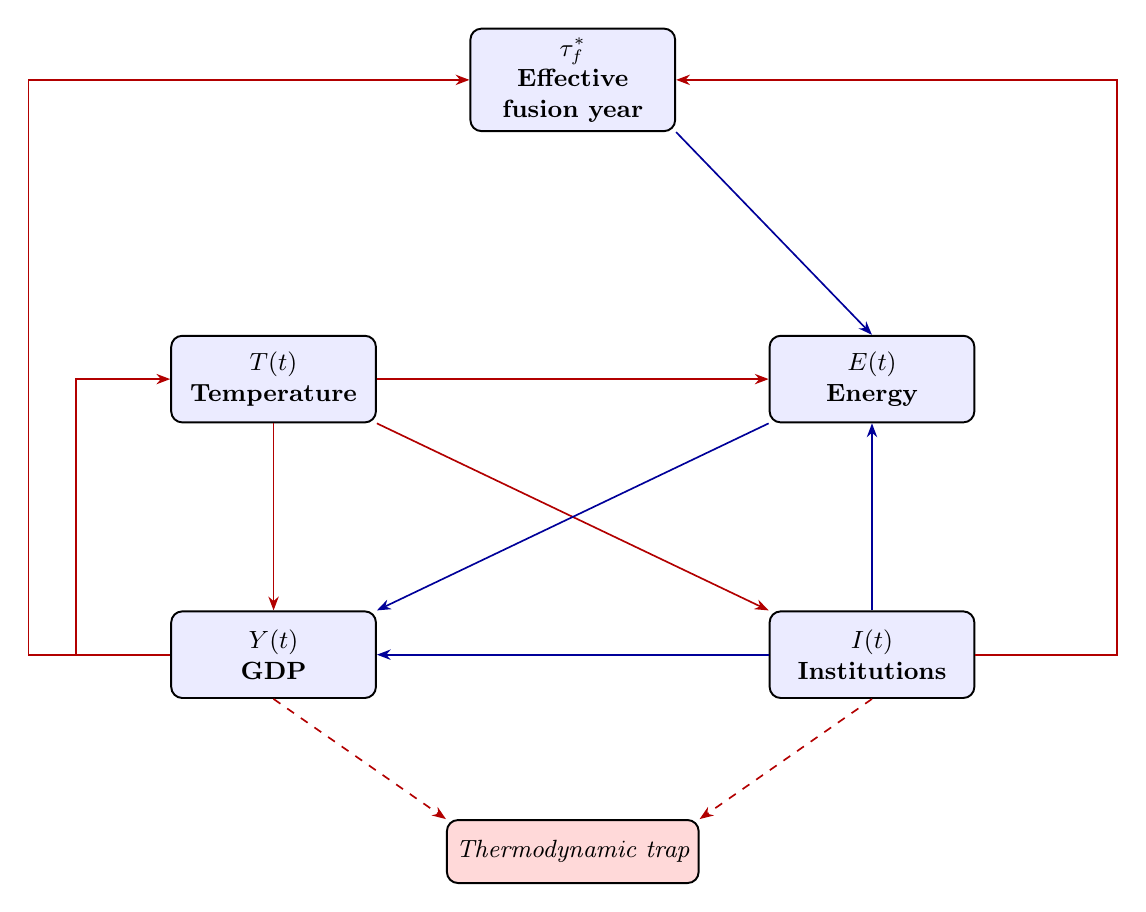
\begin{tikzpicture}[
    state/.style={draw, rounded corners, minimum width=2.6cm, minimum height=1.1cm,
                  font=\small\bfseries, fill=blue!8, align=center, line width=0.7pt},
    posarrow/.style={-{Stealth[length=5pt]}, semithick, blue!60!black},
    negarrow/.style={-{Stealth[length=5pt]}, semithick, red!70!black},
]

% --- Nodes: two rows, fusion year centered above ---
\node[state] (tau) at (0, 3.8)  {$\tau_f^*$\\Effective\\fusion year};
\node[state] (T)   at (-3.8, 0) {$T(t)$\\Temperature};
\node[state] (E)   at (3.8, 0)  {$E(t)$\\Energy};
\node[state] (Y)   at (-3.8, -3.5) {$Y(t)$\\GDP};
\node[state] (I)   at (3.8, -3.5)  {$I(t)$\\Institutions};

% --- Thermodynamic trap ---
\node[draw, rounded corners, fill=red!15, font=\small\itshape,
      minimum width=2.8cm, minimum height=0.8cm, line width=0.7pt] (trap) at (0, -6) {Thermodynamic trap};

% ===================== EDGES =====================

% Fusion year -> Energy (positive: fusion ramp)
\draw[posarrow] (tau.south east) -- (E.north);

% Temperature -> Energy (negative: EROI decay)
\draw[negarrow] (T.east) -- (E.west);

% Temperature -> GDP (negative: damages)
\draw[negarrow] (T.south) -- (Y.north);

% Temperature -> Institutions (negative: stress)
\draw[negarrow] (T.south east) -- (I.north west);

% Energy -> GDP (positive: E/15 multiplier)
\draw[posarrow] (E.south west) -- (Y.north east);

% Institutions -> GDP (positive: governance)
\draw[posarrow] (I.west) -- (Y.east);

% Institutions -> Energy (positive: enables clean energy & fusion adoption)
\draw[posarrow] (I.north) -- (E.south);

% GDP -> Temperature (negative: emissions) — routed outside left
\draw[negarrow] (Y.west) -- ++(-1.2, 0) |- (T.west);

% GDP -> Fusion year (negative: low Y delays R&D) — routed outside far left
\draw[negarrow] (Y.west) -- ++(-1.8, 0) |- (tau.west);

% Institutions -> Fusion year (negative: low I delays R&D) — routed outside far right
\draw[negarrow] (I.east) -- ++(1.8, 0) |- (tau.east);

% GDP -> Trap (dashed)
\draw[negarrow, dashed] (Y.south) -- (trap.north west);

% Institutions -> Trap (dashed)
\draw[negarrow, dashed] (I.south) -- (trap.north east);

\end{tikzpicture}
\caption{Causal structure of the simulation model. \textcolor{blue!60!black}{\textbf{Blue}} arrows denote positive (reinforcing) effects; \textcolor{red!70!black}{\textbf{red}} arrows denote negative (degrading) effects. Dashed arrows indicate pathways into the absorbing thermodynamic trap. Key feedback loops: temperature degrades energy, institutions, and GDP; GDP drives emissions that raise temperature; declining GDP and institutions delay fusion R\&D; institutions modulate both pre-fusion clean energy deployment and post-fusion adoption.}
\label{fig:causal}
\end{figure}

To quantify the dynamics described above, we construct a stochastic simulation model with five coupled state variables evolving over the period 2026--2100.

\subsection{State Variables}

\begin{itemize}[leftmargin=2em]
    \item $T(t)$: Global temperature anomaly (°C above pre-industrial). Initialized at 1.3°C (estimated current value).
    \item $E(t)$: Effective energy availability index. Initialized at 15.0 (current blended EROI proxy).
    \item $Y(t)$: Global GDP in trillions of 2026 PPP dollars. Initialized at 105.0 (approximate current value).
    \item $I(t)$: Institutional stability index $\in [0, 1.2]$. Initialized at 1.0. This composite variable proxies for the aggregate capacity of governance, legal, financial, and logistical institutions to coordinate complex economic activity. A value of 1.0 represents the current institutional baseline; values above 1.0 (up to 1.2) allow for modest institutional improvement under favorable conditions (e.g., post-fusion coordination gains); values approaching 0 represent institutional collapse (failed states, broken supply chains, loss of rule of law, pervasive armed conflict). The index is deliberately abstract: it aggregates phenomena as diverse as regulatory coherence, contract enforcement, central bank credibility, port throughput, and the functioning of peer review. The justification for treating these as a single scalar is that they are \emph{correlated in practice}---institutional failures cascade through interdependent systems in much the same way as the EROI percolation threshold described in Section~2. The bounded range $[0, 1.2]$ reflects the empirical observation that institutional quality has a low ceiling (institutions improve slowly) but no floor (they can collapse rapidly).
    \item $\tau_f$: Fusion commercialization year (stochastic, drawn per path). This represents not the date of first ignition but the year at which fusion begins contributing meaningfully to global energy supply, as discussed in Section~\ref{sec:why_fusion}.
\end{itemize}

\subsection{Dynamics}

\paragraph{Temperature.} Temperature evolves as:
\begin{equation}
    \Delta T(t) = \left[0.04 \cdot \left(1 - 0.018(t - t_0)\right) \cdot \frac{Y(t)}{100} \cdot \frac{s}{3.0} \cdot \frac{15}{E(t)}\right] + \epsilon_T
\end{equation}
where $s \sim \mathcal{N}(3.0, 0.4)$ is climate sensitivity and $\epsilon_T \sim \mathcal{N}(0, 0.04)$ is stochastic variability. The $(1 - 0.018(t-t_0))$ term captures gradual exogenous decarbonization (efficiency improvements, renewable deployment). The $15/E(t)$ term captures the endogenous decarbonization effect of fusion: as energy availability $E$ rises from its pre-fusion baseline of $\sim$15 toward 100, emissions intensity per unit of GDP falls proportionally, reflecting the displacement of fossil fuels by clean energy. This ensures that fusion-powered economic growth does not produce runaway warming---the central physical rationale for fusion as a climate solution.

\paragraph{Energy.} Before fusion ($t < \tau_f^*$), energy availability declines under climate stress but is partially offset by pre-fusion clean energy deployment (solar, wind, fission, geothermal):
\begin{equation}
    E(t+1) = \max\left(1.0,\; E(t) - 0.12 - 0.03T(t) + \underbrace{\frac{c}{1 + e^{-0.15(t - 2030)}} \cdot I(t)}_{\text{pre-fusion clean energy}} + \epsilon_E\right)
\end{equation}
where $c = 0.08$ is the clean energy ceiling---calibrated so that at full adoption and institutional health, pre-fusion renewables and fission offset roughly two-thirds of the baseline EROI decay rate (0.12/yr), slowing the decline but not reversing it. This is consistent with the system-level EROI analysis in Section~\ref{sec:why_fusion}: existing low-carbon technologies can extend the window but cannot, by themselves, provide the step-change in energy surplus needed to escape the thermodynamic trap. The logistic adoption curve centered on 2030 reflects the current rapid scaling of solar and wind capacity, and the $I(t)$ multiplier ensures that institutional degradation also hampers renewable deployment.

After fusion ($t \geq \tau_f^*$), energy ramps along a logistic adoption curve:
\begin{equation}
    E(t+1) = \min\left(100,\; E(t) + 3.5 \cdot I(t) \cdot \sigma(t)\right), \quad \sigma(t) = \frac{1}{1 + e^{-k(t - t_{\text{mid}})}}
\end{equation}
where $k = 0.5$ is the adoption steepness and $t_{\text{mid}} = \tau_f^* + \ln(999)/k$ is chosen so that $\sigma(\tau_f^*) = 0.001$---i.e., fusion contributes only 0.1\% of its potential at the year of first commercialization, reaching 50\% adoption $\sim$14 years later. This captures the reality that commercial viability does not imply instant fleet deployment: manufacturing scale-up, grid integration, regulatory approval, and site construction impose an irreducible lag. The $I(t)$ multiplier ensures that institutional collapse can further slow adoption even along the S-curve.

\paragraph{Endogenous fusion delay.} The effective fusion year $\tau_f^*$ is not fixed but responds endogenously to economic and institutional conditions:
\begin{equation}
    \tau_f^*(t) = \tau_f + \sum_{s < t} \left[\max(0,\, 1 - I(s)) \cdot 0.5 + \max\left(0,\, 1 - \frac{Y(s)}{Y_0}\right) \cdot 0.5\right]
\end{equation}
where $\tau_f$ is the best-case fusion year drawn at path initialization and $Y_0 = 105$ is the initial GDP baseline. The delay accumulates only in years before fusion arrives: each year in which institutional capacity or GDP is below baseline pushes the effective commercialization date further into the future. This captures the paper's central feedback loop in the fusion timeline itself---the same climate-driven degradation that makes fusion more urgent also makes it harder to develop. When $I = 1$ and $Y = Y_0$ (no degradation), the delay is zero and fusion arrives at its best-case date. In severely degraded paths ($I \approx 0.5$, $Y \approx 50$T), the delay can accumulate at $\sim$0.5 years per year, potentially pushing fusion commercialization back by a decade or more. Note that in the causal intervention analysis (Section~\ref{sec:results_gradient}), the endogenous delay is disabled: the do-calculus framework requires fixing $\tau_f$ exogenously to isolate its causal effect.

\paragraph{Institutional Stability.} Institutions degrade under climate stress, energy scarcity, and economic volatility:
\begin{equation}
    I(t+1) = \text{clip}\left(I(t) - 0.035 \cdot L(t) + 0.006,\; 0,\; 1.2\right)
\end{equation}
where $L(t) = \frac{D(t)}{Y(t)+5} + \frac{6}{E(t)} + 8 \cdot v(t)$ aggregates damage pressure, energy scarcity, and economic velocity shocks $v(t) = \max(0, Y(t-1) - Y(t)) / (Y(t) + 10)$.

\paragraph{Collapse.} When institutional stability falls below a path-specific brittleness threshold $\beta \sim \text{Uniform}(0.1, 0.25)$, systemic collapse becomes possible with probability $0.02 + 0.2(\beta - I)$ per year. It is important to distinguish this collapse mechanism from the gradual regression to a ``physiocratic'' state that the model already captures through declining EROI and the survival basket tax. Physiocratic regression is severe but in principle reversible: a society that has lost its semiconductor fabs and research universities could, given sufficient time and external assistance, rebuild them. Systemic collapse, by contrast, represents events that are \emph{irreversible on multi-decadal timescales}: nuclear exchange between resource-stressed powers (the UK national security assessment flags Himalayan glacier loss as a plausible trigger for escalation between India, China, and Pakistan \citep{ukjic2025biodiversity}); cascading state failure across interconnected regions that destroys the global trade networks on which complex manufacturing depends; pandemic emergence from ecosystem disruption compounded by degraded public health infrastructure; or the permanent loss of critical tacit knowledge and precision manufacturing capacity when the last generation of specialists in key disciplines retires or disperses without successors. The common feature is that these events destroy not merely output but the \emph{preconditions for recovery}---the knowledge, institutions, supply chains, and trust networks that would be required to rebuild. In the model, collapse sets $Y(t)$ to 1\% of its pre-collapse value, representing not merely a GDP shock but a civilizational discontinuity from which the simulation paths almost never recover.

\paragraph{GDP.} Output evolves as:
\begin{equation}
    Y(t+1) = Y(t) + \underbrace{Y(t) \cdot g \cdot I(t) \cdot \frac{E(t)}{15} \cdot \phi(Y)}_{\text{gross growth}} - \underbrace{D(t)}_{\text{damages}} - \underbrace{M(t)}_{\text{maintenance}}
\end{equation}
where $g \sim \mathcal{N}(0.028, 0.006)$ is the base growth rate, $D(t) = 0.003 \cdot T^{2.6} \cdot Y$ captures nonlinear climate damages (as a fraction of GDP, consistent with the empirical damage function literature), $M(t) = 0.022 \cdot Y \cdot (T/1.3) \cdot e(E)$ is the survival basket maintenance cost (also as a fraction of GDP), and $\phi(Y) = 1/(1 + (Y/2000)^2)$ is a logistic growth dampener reflecting diminishing returns at high output levels.

\paragraph{A note on model structure.} This is a \emph{reduced-form GDP dynamics} equation, not a capital accumulation identity. All three terms---gross growth, damages, and maintenance---are calibrated as fractions of current GDP: $g \approx 0.028$ is the observed global GDP growth rate, the damage coefficient $0.003 \cdot T^{2.6}$ is calibrated to empirical GDP damage functions \citep{burke2015global, howard2017few}, and the maintenance rate of 0.022 reflects the survival basket tax as a share of output. The update rule is equivalent to $Y(t+1) = Y(t) \cdot (1 + r_{\text{net}}(t))$ where $r_{\text{net}}$ is the net GDP growth rate after climate damages and maintenance costs. We do not model the capital stock or the investment-to-output transmission mechanism (i.e., the incremental capital-output ratio) separately; the base growth rate $g$ implicitly absorbs the savings rate and capital productivity. This reduced-form approach is appropriate for a model whose purpose is to characterize the \emph{qualitative topology} of the feedback loop between energy surplus, climate damage, and innovation capacity, rather than to produce point forecasts of GDP levels.

\paragraph{EROI as a continuous variable.} A crucial methodological point: the model does \emph{not} impose hard EROI thresholds as exogenous assumptions. The energy variable $E$ enters the dynamics as a \emph{continuous} multiplier through three channels simultaneously: growth capacity scales as $E/15$, emissions intensity scales as $15/E$, and institutional stress includes a $6/E$ term. No single threshold is assumed. Instead, the \emph{interaction} of these continuous effects produces emergent threshold-like behavior: as $E$ declines, growth falls, emissions rise, and institutional stability erodes, each reinforcing the others. The result is a phase transition that arises from the model's dynamics rather than being imposed on them. The empirical thresholds identified by \citet{lambert2014energy} (Section~2) serve as calibration targets---they tell us that the model's emergent behavior should produce qualitative regime changes in roughly the right EROI range---but the thresholds themselves are outputs, not inputs, of the simulation.

\subsection{Stochastic Parameters}

Each of the 10,000 Monte Carlo paths draws four latent parameters:

\begin{table}[H]
\centering
\begin{tabular}{lll}
\toprule
\textbf{Parameter} & \textbf{Distribution} & \textbf{Interpretation} \\
\midrule
Best-case fusion year $\tau_f$ & $\mathcal{N}(2035, 7)$ & Year of first commercial fusion reactor \\
Climate sensitivity $s$ & $\mathcal{N}(3.0, 0.4)$ & °C per doubling of CO$_2$ \\
Brittleness $\beta$ & $\text{Uniform}(0.1, 0.25)$ & Institutional fragility threshold \\
Base growth $g$ & $\mathcal{N}(0.028, 0.006)$ & Underlying economic growth rate \\
\bottomrule
\end{tabular}
\caption{Stochastic parameters drawn independently for each simulation path.}
\label{tab:params}
\end{table}

\section{Results}

\subsection{Aggregate Outcomes}

Across 10,000 simulation paths, we classify terminal outcomes into three regimes. \emph{Abundance} denotes paths reaching $>$500T GDP by 2100---roughly 5$\times$ current global output, sufficient to sustain universal high-technology living standards and continued frontier R\&D. \emph{Systemic collapse} denotes paths where GDP falls below 1\% of its 2026 baseline, representing irreversible civilizational failure. \emph{Never recovered} denotes paths that remain below the 2026 baseline at century's end, indicating prolonged civilizational decline without outright collapse. The 500T threshold is not arbitrary: it approximates the output level at which per-capita GDP (assuming $\sim$10 billion population) exceeds \$50,000---the empirical range above which societies reliably sustain broad-based innovation ecosystems, universal higher education, and comprehensive healthcare.

\begin{table}[H]
\centering
\begin{tabular}{lr}
\toprule
\textbf{Outcome} & \textbf{Value} \\
\midrule
Uninterrupted growth (no downturn) & $\sim$3\% of paths \\
Abundance ($>$500T GDP by 2100) & $\sim$50\% of paths \\
Systemic collapse ($<$1\% of baseline) & $<$1\% of paths \\
Never recovered by 2100 & $\sim$25\% of paths \\
Median nadir year & $\sim$2059 \\
Median recovery time & $\sim$39 years \\
\bottomrule
\end{tabular}
\caption{Summary statistics from 10,000 Monte Carlo paths (2026--2100).}
\label{tab:results}
\end{table}

These results speak directly to the debate outlined in the Introduction. The Polyannaists are not wrong: $\sim$3\% of paths experience no downturn at all, vindicating the view that sociotechnical systems \emph{can} absorb climate shocks without disruption. The ecologists are also not wrong: one-quarter of paths never recover, and a small fraction experience outright civilizational collapse, vindicating the view that decline is a real and non-negligible possibility. Both camps are \emph{plausibly right}---the question is which draws from the parameter space we actually inhabit.

But the most important finding is what lies between these extremes. The vast mass of outcomes---the remaining $\sim$72\% of paths---follows a characteristic arc: \emph{it gets worse, then it gets better}. GDP declines from current levels, reaches a nadir, and then recovers (or fails to). The depth of the trough, the year of the nadir, and the speed of recovery are all overwhelmingly determined by a single variable: the timing of fusion commercialization.

This ``worse then better'' middle ground is precisely the territory that neither the Polyannaists nor the ecologists occupy, and it is where policy has the most leverage. The Polyannaist error is assuming the recovery is automatic; the ecologist error is assuming the decline is terminal. The simulation shows that the outcome is \emph{contingent}---and contingent on a variable that is, at least in principle, subject to deliberate acceleration.

\subsection{The Fusion Frontier}

Figure~\ref{fig:simulation} (top left) displays the GDP percentile fan chart with the \emph{fusion frontier} overlaid. The frontier maps each percentile of final GDP outcome to the average fusion year of paths in that percentile band. The resulting curve cuts diagonally across the fan chart, demonstrating that fusion timing is the primary axis of variation in long-run outcomes.

Paths with fusion arriving before $\sim$2035 overwhelmingly achieve abundance. Paths with fusion after $\sim$2050 overwhelmingly fail to recover. The transition zone between these regimes is remarkably narrow---approximately 15 years---underscoring the criticality of the current decade for fusion investment.

\subsection{Sensitivity Analysis}

Spearman rank correlation between each stochastic parameter and final GDP (Figure~\ref{fig:simulation}, top center) reveals a clear hierarchy:

\begin{enumerate}[leftmargin=2em]
    \item \textbf{Fusion year} ($\rho \approx -0.45$): The strongest predictor by a wide margin. Earlier fusion $\rightarrow$ higher GDP.
    \item \textbf{Climate sensitivity} ($\rho \approx -0.15$): Higher sensitivity $\rightarrow$ lower GDP, but substantially less influential than fusion timing.
    \item \textbf{Brittleness} ($\rho \approx -0.05$): Modest negative effect.
    \item \textbf{Base growth} ($\rho \approx +0.30$): Higher baseline growth helps, but cannot compensate for late fusion.
\end{enumerate}

The dominance of fusion timing over climate sensitivity is a key finding. It implies that \emph{the most effective climate policy is energy policy}---specifically, accelerating fusion commercialization. Even in high-sensitivity climate scenarios, early fusion produces favorable outcomes; conversely, even in low-sensitivity scenarios, late fusion produces poor outcomes.

\paragraph{Quantifying the fusion timing gradient.}\label{sec:results_gradient} To move beyond rank correlations, we estimate the \emph{causal} effect of fusion timing on terminal GDP using a do-calculus approach: for each target fusion year $\tau_f \in \{2026, 2030, 2035, \ldots, 2060\}$, we fix $\tau_f$ to that value and draw all other parameters (climate sensitivity, brittleness, base growth) from their baseline distributions, running 10,000 paths per intervention. This isolates the causal effect of fusion timing from any confounding correlation with other parameter draws (Figure~\ref{fig:gradient}).

\begin{figure}[H]
    \centering
    \includegraphics[width=\textwidth]{figures/gradient_plot.pdf}
    \caption{Causal effect of fusion timing on mean terminal GDP (left axis, blue), probability of abundance ($>$500T GDP, green), and probability of collapse (red). Each point fixes $\tau_f$ to the indicated year and draws all other parameters from their baseline distributions (10,000 paths per intervention). The shaded region marks the critical transition zone.}
    \label{fig:gradient}
\end{figure}

The relationship is monotonically decreasing and strikingly nonlinear. Earlier fusion is always better: $\text{do}(\tau_f = 2026)$ yields mean GDP of $\sim$2,130T with 96\% probability of abundance, while $\text{do}(\tau_f = 2060)$ yields only 2T with 20\% probability of collapse---effectively civilizational ruin. The transition is remarkably sharp: P(Abundance) drops from 96\% to near zero between 2026 and 2045, while P(Collapse) rises from zero to 20\% between 2045 and 2060. The GDP gradient is already steep at the earliest point we can measure: $\sim$130 T/yr between 2026 and 2030, peaking at $\sim$158 T/yr around 2032, and remaining above 100 T/yr through 2038. The window is not approaching---it is already open, and has likely been open for several years. After 2045, the gradient flattens ($\sim$8 T/yr between 2042 and 2048)---not because delay has become less harmful, but because most of the damage has already been done and the economy has already entered the trap.

Note that fusion simultaneously provides two benefits: it accelerates GDP growth (through the $E/15$ multiplier on investment) and it \emph{decarbonizes} the economy (emissions intensity scales as $15/E$, so a fusion-powered economy with $E \approx 100$ emits at $\sim$15\% of pre-fusion intensity per unit of output). This means early fusion does not merely grow the economy faster---it arrests the temperature trajectory that would otherwise destroy it.

\subsection{Crisis Dynamics}

The distribution of nadir years (Figure~\ref{fig:simulation}, bottom left) peaks around 2050--2065, corresponding to the period of maximum stress before fusion deployment can take effect. This is the period during which the survival basket tax is highest and institutional stability is most fragile.

Recovery times (Figure~\ref{fig:simulation}, bottom center) show a characteristic pattern: paths that recover at all tend to do so within 25--40 years of their nadir, driven by the rapid GDP growth that fusion energy enables. The sharp spike at short recovery times reflects paths where fusion arrives early enough to prevent deep downturns entirely.

\subsection{Terminal GDP Distribution}

The distribution of GDP in 2100 (Figure~\ref{fig:simulation}, bottom right) exhibits heavy left-skew with a concentration of mass near zero (collapsed paths) and a long right tail extending to $\sim$1,500T. The growth dampener $\phi(K)$ constrains the right tail to physically plausible levels while preserving the qualitative bimodality of outcomes.

\begin{figure}[H]
    \centering
    \includegraphics[width=\textwidth]{figures/simulation.pdf}
    \caption{Stochastic simulation results (10,000 paths, 2026--2100). \textbf{Top left:} GDP percentile fan chart (10th--90th) with fusion frontier. \textbf{Top center:} Spearman rank correlation of stochastic parameters with 2100 GDP. \textbf{Top right:} Distribution of minimum GDP recorded per path. \textbf{Bottom left:} Distribution of nadir year. \textbf{Bottom center:} Distribution of recovery time to baseline. \textbf{Bottom right:} Distribution of terminal GDP.}
    \label{fig:simulation}
\end{figure}

\section{Related Work}

The arguments developed in this paper draw on and extend several distinct literatures. We situate our contribution relative to each.

\subsection{EROI and Biophysical Economics}

The foundational work on EROI thresholds and their societal implications is due to \citet{hall2014eroi} and \citet{lambert2014energy}, who established the empirical link between energy surplus and the complexity of economic activity a society can sustain. \citet{brockway2019estimation} extended this analysis to global final-stage EROI, documenting the long-run decline in fossil fuel returns. Our contribution is to embed these static thresholds in a \emph{dynamic} model where EROI interacts with climate damage and institutional capacity over time, producing path-dependent outcomes rather than fixed equilibria.

The biophysical economics tradition more broadly---associated with \citet{georgescuroegen1971entropy}, \citet{daly1977steady}, and \citet{odum1971environment}---has long argued that economic models ignoring thermodynamic constraints are fundamentally incomplete. Our model operationalizes this critique in a specific, quantitative way: the EROI threshold is not merely a theoretical concern but a parameter that determines whether the innovation ecosystem survives.

\subsection{Climate Damage Functions}

The quadratic (or higher-order polynomial) damage function relating temperature to GDP loss has a long history in integrated assessment models (IAMs), beginning with Nordhaus's DICE model \citep{nordhaus2017revisiting}. \citet{burke2015global} provided influential empirical support for nonlinear damages, estimating that economic output peaks at moderate temperatures and declines sharply thereafter. \citet{howard2017few} conducted a meta-analysis finding that damage estimates are systematically higher when nonlinear specifications are used. Our damage exponent of 2.6 is calibrated to the upper range of these estimates, reflecting the view that IAM damage functions have historically been conservative, particularly at high temperature anomalies.

Unlike standard IAMs, our model does not optimize over an emissions pathway. Instead, it treats emissions as endogenous to economic activity and focuses on the \emph{consequences} of damage accumulation for innovation capacity---a channel that IAMs typically ignore or treat as exogenous.

\subsection{IPCC Shared Socioeconomic Pathways}

The IPCC's Shared Socioeconomic Pathways \citep[SSPs;][]{oneill2014new} represent the current standard framework for scenario-based climate analysis. The five SSPs (SSP1 through SSP5) span a range of assumptions about population, economic growth, inequality, governance, and technology, producing divergent emissions and adaptation trajectories. SSP1 (``Sustainability'') assumes rapid decarbonization and strong international cooperation; SSP5 (``Fossil-fueled Development'') assumes continued high growth powered by fossil energy; SSP3 (``Regional Rivalry'') assumes fragmentation and slow development.

Our model departs from the SSP framework in a fundamental way. The SSPs treat socioeconomic trajectories as \emph{exogenous scenarios}---narrative assumptions that drive emissions, which in turn drive climate outcomes. The feedback from climate outcomes back to socioeconomic trajectories is largely absent or handled through separate damage overlays. In our model, by contrast, the socioeconomic trajectory is \emph{endogenous}: GDP, institutional stability, and energy availability co-evolve with temperature, and the feedback from climate damage to innovation capacity is the central mechanism.

This distinction matters because the SSP framework implicitly assumes that the socioeconomic narrative chosen at the outset persists through the century. SSP1 assumes that the institutions and capital required for sustainability \emph{remain available} throughout the transition. SSP3 assumes fragmentation without asking whether fragmentation might be a \emph{consequence} of the climate trajectory rather than an independent assumption. Our model shows that these are not independent axes: a society that begins on an SSP1-like trajectory can be pushed onto an SSP3-like trajectory by the interaction of climate damage and institutional erosion, and the variable that most determines which trajectory prevails is the timing of energy transition---specifically, fusion commercialization.

The SSP framework is also silent on the possibility of \emph{threshold effects} in the socioeconomic domain. Our model's collapse dynamics---where institutional stability falls below a brittleness threshold and triggers cascading failure---have no analogue in the SSP narratives, which assume smooth evolution along their respective trajectories. The simulation results suggest that this omission may be consequential: approximately 1\% of paths experience outright systemic collapse, a possibility that the SSP framework does not contemplate.

\subsection{Institutional Fragility and Collapse}

The modeling of institutional stability as a threshold-dependent variable draws on the complex systems literature on cascading failures \citep{albert2000error}, on recent arguments that catastrophic climate scenarios are dangerously underexplored \citep{kemp2022climate, richards2022climate}, and on historical analyses of civilizational collapse. \citet{tainter1988collapse} argues that societies collapse when the marginal returns to complexity become negative---a framing closely related to our EROI threshold argument. \citet{diamond2005collapse} documents environmental overshoot as a recurring driver of institutional failure.

More recently, the political science literature on state fragility \citep[e.g., the Fragile States Index;][]{fundforpeace2023fsi} has documented the empirical correlation between climate stress, resource scarcity, and institutional degradation. The 2025 UK national security assessment on biodiversity loss and ecosystem collapse \citep{ukjic2025biodiversity} goes further, concluding that ecosystem degradation is now a strategic security threat that will drive ``conflict and military escalation \ldots both within and between states, as groups compete for arable land and food and water resources''---precisely the institutional destabilization pathway our model captures through the $I(t)$ dynamics. Our institutional stability index is a stylized representation of these dynamics, deliberately reduced to a single scalar to maintain tractability while capturing the essential feedback between environmental stress and governance capacity.

\subsection{Ruin, Irreversibility, and Ergodicity}

Our model's collapse dynamics connect to a broader theoretical literature on ruin as an absorbing barrier. \citet{taleb2014precautionary} formalize the distinction between risks that are \emph{recoverable} (local, bounded, and reversible) and risks that entail \emph{ruin} (systemic, irreversible, and total). Their central argument is that when a system faces even a small probability of ruin per unit time, the cumulative probability of ruin approaches certainty over long horizons---ruin is an absorbing state from which no recovery is possible. This is the mathematical basis of the Precautionary Principle: for ruin-class risks, expected-value reasoning is inadequate because the ensemble average (across parallel worlds) diverges from the time average (the single trajectory actually experienced by the system). \citet{peters2019ergodicity} develop this insight into a general framework---ergodicity economics---showing that the standard expected utility approach systematically underestimates the cost of irreversible losses because it implicitly assumes ergodicity (that time averages equal ensemble averages), an assumption that fails precisely when absorbing barriers exist.

Our simulation instantiates this framework concretely. The ``thermodynamic trap'' is an absorbing basin: once the system enters it---once EROI, institutional capacity, and capital have degraded past the point where fusion development is feasible---no endogenous mechanism restores the system to its prior state. The 25\% of paths that never recover by 2100 are not merely unlucky draws that will eventually revert to the mean; they are trapped in a basin from which the mean is unreachable. This is ruin in Taleb's precise sense.

The irony is that Taleb and his co-authors typically invoke the ruin framework to justify the Precautionary Principle as a \emph{constraint on action}---arguing that novel technologies with systemic risk profiles (GMOs, certain AI applications, gain-of-function research) should be restricted because their tail risks are ruinous and irreversible. Our model inverts this logic. In the closing window framework, the ruinous absorbing barrier is not a consequence of reckless technological action but of \emph{insufficient} technological action. The ruin state is not ``we built fusion and something went catastrophically wrong''; it is ``we failed to build fusion in time and the innovation ecosystem collapsed.'' Inaction---or insufficiently aggressive action---is the policy that maximizes the probability of ruin. The Precautionary Principle, correctly applied to a system with the feedback topology we describe, demands not caution but urgency: the greatest systemic risk is the risk of delay.

This reframing also clarifies why standard cost-benefit analysis (CBA) of fusion investment is inadequate. CBA operates on ensemble averages---it asks ``what is the expected return across all possible futures?'' But as Peters and Taleb emphasize, an agent who exists in \emph{time} (not across parallel worlds) should maximize the time-average growth rate, which penalizes ruin far more heavily than the ensemble average does. The social ROI figures reported in Section~9 are already extraordinary under ensemble averaging; under time-average reasoning, the case for aggressive fusion investment is stronger still, because the cost of the ruin paths is not merely a probability-weighted loss but an \emph{existential} one.

\subsection{Fusion Energy Economics and Timelines}

\citet{cabal2017fusion} analyzed fusion's potential role in future low-carbon electricity systems, finding that fusion could contribute significantly to baseload generation if commercialized by mid-century. More recently, \citet{schwartz2023value} modeled fusion's economic value in a decarbonized U.S.\ grid, finding that competitive fusion plants could reduce system costs by hundreds of billions of dollars, and \citet{armstrong2024role} concluded that fusion could reduce the global cost of decarbonization by trillions under favorable cost assumptions. The fusion timeline literature is extensive and contentious; our distribution $\tau_f \sim \mathcal{N}(2035, 7)$ reflects the current wave of private-sector timelines targeting first commercial reactors in the early 2030s \citep{creely2020overview, wurzel2022progress}, while the logistic adoption curve ($k = 0.5$, 50\% deployment $\sim$14 years after first commercialization) captures the irreducible lag between a working reactor and fleet-scale deployment. The historical pattern of timeline slippage is accommodated by the distribution's right tail, which places non-negligible probability on first commercialization as late as 2050.

Our contribution relative to the fusion economics literature is to model fusion not as an isolated technology deployment problem but as a \emph{race against institutional and economic degradation}---a framing that makes the timeline question existential rather than merely economic.

\subsection{Abundance Agenda and Techno-Optimism}

The ``Abundance Agenda'' (Yglesias, Thompson, Cowen, and others) and the broader techno-optimist movement argue that the primary barrier to human flourishing is not resource scarcity but institutional sclerosis---permitting failures, regulatory capture, and political dysfunction that prevent the deployment of technologies already available or nearly so. Our model is broadly sympathetic to this framing but adds a critical nuance: institutional capacity is not merely a policy variable to be optimized but is itself \emph{endogenous to environmental and economic conditions}. The Abundance Agenda is correct that institutions matter enormously, but it underestimates the degree to which institutional quality is downstream of the thermodynamic and economic conditions we model.

\subsection{Degrowth and Limits-to-Growth Traditions}

The degrowth literature \citep{kallis2018degrowth, hickel2020less, jackson2009prosperity} and its intellectual ancestor \citep{meadows1972limits} argue that indefinite economic growth on a finite planet is physically impossible and that voluntary contraction of material throughput is both necessary and desirable. Our model engages this tradition in two ways. First, the growth dampener $\phi(K)$ explicitly acknowledges diminishing returns at high GDP levels---growth does not continue exponentially forever. Second, however, the simulation results show that the degrowth scenario (paths where GDP contracts and remains low) is not a stable, desirable equilibrium but a \emph{trap}: paths that enter sustained contraction lose the capacity to develop the technologies needed to stabilize the climate, producing a vicious cycle of further degradation. Voluntary degrowth, in our framework, is strategically equivalent to closing the fusion window prematurely.

\section{Discussion}

\subsection{The Trap Geometry}

The results formalize an intuition that is difficult to express in standard economic models: civilizational progress is not guaranteed, and the conditions for continued progress are themselves fragile. The interaction of thermodynamic thresholds, the survival basket tax, and capital-dependent innovation creates a \emph{trap geometry} with the following structure:

\begin{enumerate}[leftmargin=2em]
    \item Climate damages reduce energy surplus (EROI declines).
    \item Reduced surplus shifts spending toward the survival basket.
    \item Survival basket crowding-out reduces R\&D capacity.
    \item Reduced R\&D delays fusion and other breakthrough technologies.
    \item Delayed breakthroughs allow further climate damage accumulation.
    \item Return to step 1.
\end{enumerate}

This is a positive feedback loop with a basin of attraction. Once the system enters the basin---once the R\&D Death Cross is passed---escape requires an exogenous intervention of decreasing probability. The simulation shows that approximately 25\% of paths enter this basin and never escape.

\subsection{Policy Implications}

The standard portfolio approach to climate policy---diversifying across mitigation, adaptation, and R\&D---may be inadequate if the closing window dynamic is real. The simulation results do not suggest incremental policy adjustments. They suggest a fundamental reorientation of priorities:

\begin{enumerate}[leftmargin=2em]
    \item \textbf{Fusion as critical path.} Fusion commercialization is not one item in a diversified R\&D portfolio. It is, by a wide margin, the single variable with the largest causal effect on long-run outcomes---larger than climate sensitivity, institutional quality, or baseline growth. The policy implication is not that fusion deserves \emph{more} funding, but that it deserves a categorically different level of funding, commensurate with the civilizational stakes.
    
    \item \textbf{Urgency over optimality.} The narrow transition zone ($\sim$2030--2045) means that speed of deployment matters more than cost optimization. Each year of acceleration in this window is worth thousands of trillions of dollars in cumulative output (see below). Policies that accelerate fusion by even 5 years---regulatory fast-tracking, guaranteed procurement, Manhattan Project--scale public investment---produce outsized improvements in expected outcomes.
    
    \item \textbf{Institutional resilience as insurance.} While fusion timing dominates, institutional stability determines whether a society can \emph{deploy} fusion once it is available. A society that develops commercial fusion in 2042 but has already undergone institutional collapse cannot build the reactors. Maintaining institutional capacity during the stress period is a necessary complement to fusion R\&D.
    
    \item \textbf{Survival basket mitigation.} Policies that reduce the survival basket tax---food system resilience, water infrastructure, cooling access---buy time by slowing the closure of the innovation window, even if they do not directly advance fusion. These are not alternatives to fusion investment but force multipliers for it.
\end{enumerate}

\paragraph{The case for massive investment.} The urgency of point (2) can be made precise. The social return on investment implied by these results is extraordinary---and substantially larger than the terminal GDP figures in Figure~\ref{fig:gradient} suggest. The benefit of accelerating fusion is not a lump sum realized in 2100; it is a \emph{stream} of annual GDP increments beginning at the earlier deployment date and compounding through the end of the century. Computing the full cumulative GDP gain (the integral of the trajectory difference), each year of acceleration during the high-gradient period is worth approximately 470--3,600 trillion dollar-years of cumulative output---roughly 12$\times$ the terminal-only figure. For comparison, the most expensive fusion project in history---ITER---has a total estimated construction cost of \$22 billion (EU estimate) to \$65 billion (U.S.\ DOE estimate including in-kind contributions).\footnote{ITER cost estimates vary by accounting methodology. The European estimate of ${\sim}$EUR~22 billion covers direct construction; the U.S.\ Department of Energy's estimate of \$65 billion includes in-kind contributions from all member nations. See \url{https://www.iter.org/faqs}.} Even at the upper bound, ITER's \emph{entire lifetime cost} is less than 2\% of the cumulative GDP at stake from a single year of delay.

A generous upper bound on total cumulative global fusion capex---ITER, all national programs, and all private investment since the 1950s---is approximately \$100 billion. Discounting the cumulative GDP gain stream yields a present value per year of acceleration that dwarfs this figure at every discount rate used in climate economics: $\sim$1,220$\times$ at the Stern Review's 1.4\%, $\sim$144$\times$ at Nordhaus's 5\%, and still 11$\times$ even at 10\%---well above any rate in the literature. The break-even discount rate, at which the present value of one year of acceleration merely \emph{equals} total historical fusion capex, is approximately 16\%: current investment levels are rational only under a discount rate that no economist has ever seriously proposed. The binding constraint on fusion investment is not money but the absorptive capacity of the research and engineering pipeline---a constraint that is itself relaxed by early, sustained funding.

An important caveat: these figures do \emph{not} imply a linear relationship between funding and acceleration. The transfer function from dollars to years-of-advancement is highly nonlinear, with hard bottlenecks in experimental iteration cycles (each tokamak or laser shot takes time regardless of budget), talent pipeline depth (plasma physicists cannot be trained in months), materials qualification (neutron damage testing requires years of irradiation), and regulatory learning curves. Doubling the budget does not halve the timeline. But the relevant question is not whether the marginal dollar buys a proportional speedup---it is whether the \emph{current} funding level is anywhere near the absorptive frontier. It is not. Global public fusion R\&D spending is approximately \$5 billion per year; private investment, while accelerating, adds perhaps \$5--7 billion more. For a technology whose acceleration by a single year is worth trillions, the system is operating deep in the regime where additional funding \emph{does} buy meaningful acceleration---through parallel experimental programs, redundant engineering approaches, expanded training pipelines, and de-risked supply chain development. The returns calculated above should be understood not as ``spend \$X, get \$Y'' but as ``the expected value of the acceleration achievable by moving from the current starvation-level funding regime to one commensurate with the stakes is extraordinarily large, even under conservative assumptions about the shape of the transfer function.''

Emerging AI-enabled strategic decision-making tools could, in principle, further relax the absorptive frontier. In \citet{walters2025gaiatt} we describe a neurosymbolic framework (the GAIA Tech Tree) designed to optimize portfolio allocation across technology pathways, identify bottleneck technologies whose acceleration would unblock entire downstream pathways, and compress the deliberation cycles that precede investment decisions. For example, the system's dependency graph reveals that investment in radiation-hardened electronics or high-temperature superconductors simultaneously accelerates multiple fusion \emph{and} fission reactor concepts---a cross-domain synergy invisible to siloed R\&D planning. Whether such tools can deliver these benefits at scale remains to be demonstrated, but the potential is significant given the extraordinary returns to even modest acceleration. More broadly, AI is beginning to accelerate fusion development directly: machine-learning-driven plasma control, surrogate models replacing expensive tokamak shots, and automated materials screening are shortening experimental iteration cycles that were previously hard bottlenecks regardless of funding level \citep{catf2024aifusion}. If these tools shift the transfer function from dollars to years-of-advancement even modestly leftward, the already extraordinary returns to fusion investment become larger still.

\paragraph{Geographic heterogeneity and global coupling.} Our model aggregates the world into a single system, but the dynamics it describes are geographically heterogeneous in some respects and globally coupled in others---and the distinction matters for policy.

The \emph{costs} of the closing window are spatially concentrated. The survival basket tax falls hardest on tropical and subtropical regions, where wet-bulb heat stress, crop yield loss, and water scarcity are most acute. Institutional fragility is concentrated in states already near the brittleness threshold---the Sahel, South Asia, Central America---where climate stress compounds pre-existing governance deficits. Coastal and low-lying regions bear disproportionate infrastructure costs. In the near term, OECD nations will experience the survival basket tax as rising food prices and insurance costs; equatorial nations will experience it as famine, displacement, and state failure.

But the \emph{innovation ecosystem} that produces fusion is irreducibly global. Semiconductor fabrication depends on lithography machines from the Netherlands, neon gas (until recently) from Ukraine, rare earth processing in China, and chip design in the United States and Taiwan. ITER---the most advanced fusion experiment in the world---is itself a monument to this interdependence: a seven-party international collaboration (EU, US, China, Russia, India, Japan, South Korea) in which no single nation possesses the full stack of capabilities required for construction, from the European-manufactured vacuum vessel to Japanese superconducting coils to Chinese magnet feedthroughs. Beyond ITER, fusion research draws on plasma physics expertise distributed across dozens of national laboratories and supply chains for exotic materials (beryllium, tungsten, tritium breeding blankets) that span the globe. The degradation of institutional capacity in \emph{any} major node of this network degrades the capacity of the \emph{entire} network. A society that believes it can insulate itself from the closing window because its own institutions remain intact misunderstands the topology: the window is not national but civilizational.

Conversely, the \emph{benefits} of fusion deployment are globally diffusive. Once commercialized, fusion reactor designs, manufacturing know-how, and operational expertise propagate through the same trade and knowledge networks that currently sustain the innovation ecosystem. The EROI restoration is a global public good: fusion deployed anywhere reduces emissions everywhere (through displacement of fossil generation) and makes the survival basket reduction technologies of Section~\ref{sec:basket_reducer} available to all. This asymmetry---locally concentrated costs, globally coupled innovation capacity, globally diffusive benefits---strengthens the case for treating fusion as a coordination problem requiring international mobilization rather than a national competitiveness play. AI-enabled tools such as the GAIA Tech Tree \citep{walters2025gaiatt} are particularly well-suited to this coordination role: by making cross-domain technology dependencies explicit and quantifiable across institutional and national boundaries, they can serve as shared epistemic infrastructure---a common operating picture for globally distributed R\&D efforts that would otherwise optimize locally within national or corporate silos.

\subsection{Limitations and the Role of Calibration Uncertainty}

A candid assessment of this model must begin with the observation that \emph{nearly every parameter is deeply uncertain}. The damage exponent of 2.6, the EROI decay rate of 0.12 per year, the institutional degradation coefficient of 0.035, the growth dampener ceiling of 2,000T---none of these are known with precision, and several are not directly measurable at all. The fusion year distribution $\mathcal{N}(2035, 7)$ is informed by current private-sector timelines that have historically proven unreliable. The institutional stability index compresses an enormous range of social, political, and logistical phenomena into a single scalar with an admittedly arbitrary bounded range.

We do not regard this as a weakness to be apologized for, but as a feature to be understood. The model is not a forecasting instrument. It does not predict that GDP will reach any particular level by 2100, that the median nadir will occur in 2059, or that 25\% of futures are unrecoverable. These numbers are outputs of a particular calibration and would change---in some cases substantially---under alternative parameter choices.

What the model \emph{does} establish is a \textbf{qualitative structural claim}: that the interaction of thermodynamic thresholds, climate-driven resource reallocation, and capital-dependent innovation creates a feedback topology with specific properties---path dependence, threshold effects, a closing window, and dominance of energy transition timing over other variables. These structural properties are robust across a wide range of calibrations. To demonstrate this concretely, Table~\ref{tab:robustness} reports key outcomes under 14 alternative calibrations, each varying a single parameter while holding the rest at baseline.

\begin{table}[H]
\centering
\small
\begin{tabular}{lrrrrr}
\toprule
\textbf{Calibration} & \textbf{Abundance} & \textbf{Never Rec.} & \textbf{Collapse} & \textbf{Med.\ GDP} & \textbf{No Downturn} \\
\midrule
Baseline & 50.6\% & 24.3\% & 0.2\% & 520T & 2.8\% \\
Damage exp = 2.0 & 65.8\% & 12.3\% & 0.0\% & 1144T & 4.8\% \\
Damage exp = 3.2 & 28.0\% & 49.3\% & 5.0\% & 92T & 1.7\% \\
EROI decay = 0.06 & 54.1\% & 20.5\% & 0.0\% & 623T & 2.9\% \\
EROI decay = 0.18 & 46.8\% & 29.4\% & 0.7\% & 400T & 2.4\% \\
Inst. coeff = 0.020 & 80.7\% & 5.6\% & 0.0\% & 1868T & 4.1\% \\
Inst. coeff = 0.050 & 22.0\% & 55.7\% & 8.0\% & 45T & 1.9\% \\
GDP ceiling = 1000T & 47.5\% & 25.0\% & 0.2\% & 440T & 2.7\% \\
GDP ceiling = 4000T & 51.1\% & 24.8\% & 0.2\% & 537T & 2.8\% \\
Fusion $\mu$ = 2028 & 80.7\% & 6.6\% & 0.0\% & 1917T & 12.7\% \\
Fusion $\mu$ = 2045 & 10.8\% & 66.3\% & 4.2\% & 22T & 0.1\% \\
\bottomrule
\end{tabular}
\caption{Robustness of key outcomes to alternative parameter calibrations (10,000 paths each). Baseline calibration shown in first row.}
\label{tab:robustness}
\end{table}


The quantitative outcomes vary substantially---median GDP in 2100 ranges from 19T (late fusion mean) to 1,911T (early fusion or low institutional fragility)---but the qualitative structure is invariant. In every calibration, a substantial fraction of paths achieves abundance, a substantial fraction never recovers, and the split between these regimes is dominated by fusion timing. The damage exponent and institutional fragility coefficient are the most influential non-fusion parameters: raising the damage exponent from 2.6 to 3.2 roughly doubles the never-recovered fraction, while lowering the institutional coefficient from 0.035 to 0.020 more than triples median GDP. But even in the most optimistic non-fusion calibrations, late fusion ($\mu = 2045$) produces median GDP of only 19T and 65\% never-recovered paths. No parameter adjustment compensates for late fusion.

The clean energy ceiling variations deserve particular attention. Even tripling the baseline ceiling from 0.08 to 0.24---implying that pre-fusion renewables could offset \emph{twice} the baseline EROI decay rate---raises median GDP only from 537T to 699T and abundance from 51\% to 56\%. The effect is modest because the clean energy contribution faces three compounding headwinds: the temperature-driven EROI decay term ($0.03 \times T$) grows over time while the ceiling is fixed; institutional degradation reduces deployment capacity (the $I(t)$ multiplier); and the logistic adoption curve means the full ceiling is not reached until the late 2030s, by which point significant EROI damage has already accumulated. This is consistent with the empirical finding of \citet{york2019energy} that renewable energy growth has historically \emph{added} to rather than \emph{displaced} fossil fuel consumption---the structural dynamics of energy systems resist simple substitution, and the net effect on blended EROI is smaller than nameplate renewable capacity would suggest. In the model, as in reality, pre-fusion clean energy buys time but does not provide escape velocity.

The specific percentages and dollar figures reported in Section~7 should therefore be read as \emph{illustrative}, not predictive. They demonstrate the shape of the outcome distribution under one plausible calibration. The policy-relevant conclusions---that fusion commercialization is the critical-path variable, that the window is narrow, and that the trap is real---follow from the model's structure, not from the precise values of its parameters.

The model also omits important dynamics: regional heterogeneity in climate impacts and institutional capacity, trade and migration as adaptive mechanisms, the possibility of multiple partial breakthroughs rather than a single fusion event, learning curves and cost dynamics in renewable deployment, and the potential for geoengineering to buy additional time. Each of these omissions could be addressed in extensions, but we believe the core structural insight---the closing window and its dependence on energy transition timing---would survive their inclusion.

\subsection{GDP PPP as a Proxy for Civilizational Capacity}

Our model uses global GDP in purchasing-power-parity (PPP) trillions as its primary state variable. This choice invites a familiar set of objections: GDP does not measure well-being, ignores distributional inequality, omits non-market goods (ecosystem services, unpaid care work, leisure), counts destructive activity (disaster cleanup, military spending) as positive output, and is blind to sustainability---an economy liquidating its natural capital registers the same GDP growth as one investing in durable prosperity. These criticisms are well-established and, in their own domains, correct \citep{stiglitz2010mismeasuring}.

We use GDP nonetheless, for three reasons.

First, our argument does not depend on GDP as a measure of \emph{welfare}. It depends on GDP as a measure of \emph{productive capacity}---specifically, the capacity to sustain complex supply chains, fund frontier R\&D, train specialized workforces, and deploy capital-intensive infrastructure. For this purpose, GDP PPP is a reasonable proxy. A civilization with 500T of annual output can build fusion reactors, semiconductor fabs, and research universities; a civilization with 5T of annual output cannot, regardless of how equitably that output is distributed or how accurately it reflects subjective well-being. The relevant question is not ``are people happy?'' but ``does the economy generate sufficient surplus to sustain the innovation ecosystem?''---and GDP, for all its flaws, tracks this quantity tolerably well.

Second, the model's dynamics are driven by \emph{ratios and growth rates}, not absolute levels. The survival basket tax operates as a share of output; the EROI multiplier scales investment as a fraction of current GDP; institutional stability degrades in proportion to damage relative to capital. These ratio-based dynamics would be structurally identical under any aggregate output metric that correlates with productive capacity---Genuine Progress Indicator (GPI), Inclusive Wealth Index (IWI), or even a composite human development measure. The feedback loops that produce the closing window---declining energy surplus $\rightarrow$ reduced investment $\rightarrow$ slower innovation $\rightarrow$ delayed energy transition $\rightarrow$ further decline---do not depend on the accounting conventions used to measure the aggregate. Replacing $Y(t)$ with any monotonic transformation of productive capacity would rescale the axis labels without altering the phase portrait.

Third, PPP adjustment addresses the most policy-relevant distortion in nominal GDP comparisons. By converting output at purchasing-power-equivalent exchange rates rather than market rates, PPP GDP better reflects the actual volume of goods and services an economy can produce and deploy domestically---which is precisely what matters for building and maintaining complex technological infrastructure. A country's ability to train engineers, pour concrete, and manufacture precision components depends on its real productive capacity, not on the dollar price of its currency.

The substantive conclusions of the model---the existence of a closing window, the dominance of fusion timing, the threshold behavior of the EROI-institution-capital feedback loop---are properties of the \emph{topology} of the dynamical system, not of the units in which its state variable is denominated. Any metric that captures ``aggregate capacity to sustain complex economic activity'' would produce the same qualitative results.

\section{Conclusion}

Modern civilization sits at a thermodynamic threshold. The energy surpluses that fund advanced research, complex supply chains, and institutional stability are being eroded by climate change through a mechanism we have called the survival basket tax. The technologies that could resolve this crisis---above all, commercial fusion energy---are themselves products of the surplus economy that climate change is degrading. The result is a closing window whose existence vindicates neither the Polyannaists nor the ecologists exclusively: the vast majority of simulation paths pass through a period where things get substantially worse before they get better, with fusion timing determining the depth and duration of the trough.

The simulation results are stark. Across every calibration we tested, fusion timing is the single strongest predictor of whether civilization reaches 2100 in a state of abundance or prolonged decline. The transition zone is narrow and we are already inside it: the cost of delay is already close to its peak, and flattens to near zero by 2045. The specific dollar figures are outputs of a loosely calibrated model---particularly the institutional fragility coefficient is extremely challenging to quantify with any precision---and should be read as indicative of scale rather than precise forecasts. However, the order of magnitude---each year of delay costing on the order of 100 trillion dollars in expected output---is robust to wide variation in parameters, and the logistic adoption curve means that even ``early'' fusion takes over a decade to reach full deployment, making the urgency of first commercialization all the greater.

The implication is not that other climate policies are unimportant, but that they are \emph{insufficient} without a breakthrough in energy supply. Adaptation buys time. Mitigation slows the damage. Pre-fusion clean energy---even at triple the baseline deployment ceiling---improves median outcomes only modestly, because the compounding temperature-driven EROI decay and institutional erosion outpace what renewables alone can offset. Only a step-change in EROI---fusion or its equivalent---provides escape velocity from the thermodynamic trap. Emerging AI capabilities---from neurosymbolic tools that optimize cross-domain R\&D portfolios \citep{walters2025gaiatt} to machine-learning systems that compress experimental iteration cycles \citep{catf2024aifusion}---offer a genuine prospect of widening the window from the inside. The social return on accelerating that step-change is, by any standard measure, the largest investment opportunity in human history.

The window is open. It will not remain so indefinitely.

\bibliographystyle{apalike}
\bibliography{references}

\end{document}
